\subsection{Initialization} % TODO: FIX THIS SECTION

Before the \textsc{Natural} system can process queries, it requires initialization
with historical data to construct a specific embedding space $v \in \mathcal{V}$ and
schema distance index $d \in \mathcal{D}$. This phase analyzes and samples existing
datasets and previous user interactions to build 
advanced example selection.

\subsubsection{Embedding}\label{design:embedding}

Building upon DAIL-SQL's masked example selection, \textsc{Natural} utilizes 
cosine similarity in an embedding space $v$ to search for examples based on the
masked natural language query $q'$ and the respective masked SQL query $\omega'$.
This allows $\sigma$ to use cosine distance to search through historically observed
question answer pairs; eg, from previous user interactions or prevalent training
datasets like \textsc{Spider}, \textsc{Bird} or \textsc{SynSQL-2.5m}.

We therefore embedd a set of masked samples $\mathcal{S}$ into an embedding space $v_{\mathcal{S}}$,
where $\mathcal{S} = \{(q_1, s_1), ..., (q_i, s_i)\}$, $q$ is the natural language
question and $s$ is the corresponding SQL query.

The embedding space $v_{\mathcal{S}}$ can be defined as:

$$v_{\mathcal{S}} = \{~(q, \iota(mask(q)), s, \iota(mask(s)))~|~(q, s) \in \mathcal{S}~\}$$

Where the masking function $mask$ is defined as described in the sections~\ref{design:nl-masking}
and~\ref{design:sql-masking} and the embedding function is defined as $\iota$.
% TODO: Specify embedding model

\paragraph{Natural Language Masking}\label{design:nl-masking}

Masking of natural language is the process of replacing all words which are not
deemed \textit{structurally relevant} with the \texttt{<mask>} token. All words
$w$ in a constant whitelist $\mathcal{W}$ are determined structurally relevant.
% TODO: Fix typo
Estimating a constant $\mathcal{W}$ is described in section~\ref{implementation:whitelisting}.
% TODO: Fix reference to implementation section

Working with masked language enables the system to capture semantic patterns
independently of domain terminology, improving the generalizability across
domains.

Given $\mathcal{W} = \{\text{list}, \text{show}, \text{all}, \text{the},
\text{with}\}$ the natural language
questions:

\begin{verbatim}
Show all customers with the firstname John
List all products with the name iPhone
\end{verbatim}

Will get masked into the same sentence, such that the semantic words are
maintained, but domain specific terminology is discarded:

\begin{verbatim}
Show all <mask> with the <mask> <mask>
\end{verbatim}

\paragraph{SQL Masking}\label{design:sql-masking}

Masking SQL queries refers to transforming all identifiers contained in 
a SQL query to \texttt{<mask>} and all value literals to \texttt{<value>}.

Thus, the queries:

\begin{verbatim}
SELECT * FROM customers WHERE firstname = 'John'
SELECT * FROM products WHERE name = 'iPhone'
\end{verbatim}

get masked to:

\begin{verbatim}
SELECT * FROM <mask> WHERE <mask> = <value>
\end{verbatim}

% TODO: Discuss potential limitations of masked embedding approach

% ALIGNMENT IMPROVEMENTS NEEDED:
% TODO: Add formal mathematical definition using enumerate style like indexing section
% TODO: Use consistent tuple notation (q,s,ω,d) matching definitions section  
% TODO: Add cross-references to Section~\ref{design:indexing} for schema distances
% TODO: Include similarity scoring methodology with weights w_q, w_s, w_sql
% TODO: Add subsection on "Distance Calculation" parallel to indexing section
% TODO: Use consistent variable naming (mathcal{V} vs V vs v)
% TODO: Add example showing multi-dimensional scoring like indexing graphs
% TODO: Include legend/explanation of masking tokens like indexing legend

\subsubsection{Schema Indexing}

To choose the most relevant subset of samples for few-shot learning,
it is important that the SQL queries we choose as examples are written for
structurally similar database schemas in order to minimize the structural
difference between the selected samples and the ground truth query for a given
natural language question.

For example $\omega_{ground}$ the question ``Give me all contacts for the user with the id 10''
might look different depending on the database schema at hand, thus only selecting
samples based on the similarity of the natural language question will yield inferior
sample quality.

\begin{figure}[ht]
  \vspace{1em}
  \hfill
  \begin{minipage}[b]{0.45\linewidth}
    \begin{verbatim}
CREATE TABLE users (
  id TEXT PRIMARY KEY
);

CREATE TABLE contacts (
  user_id TEXT NOT NULL,
  name TEXT NOT NULL,
  FOREIGN KEY (user_id) 
   REFERENCES users(id),
  PRIMARY KEY (user_id, name)
);
    \end{verbatim}
    \caption{Normalized schema}
    \label{figure:schema-normalized}
  \end{minipage}
  \hfill
  \begin{minipage}[b]{0.35\linewidth}
    \begin{verbatim}
CREATE TABLE users (
  id TEXT PRIMARY KEY,
  contacts TEXT[] NOT NULL
);
    \end{verbatim}
    \vspace{3.75em}
    \caption{Denormalized schema}
    \label{figure:schema-denormalized}
  \end{minipage}
  \hfill
  \vspace{1em}
\end{figure}

Given the database schemas in figures~\ref{figure:schema-normalized} and~\ref{figure:schema-denormalized}
respective definitions of $\omega_{ground}$ would be~\ref{figure:sql-join-example}
and~\ref{figure:sql-array-example}.

\begin{figure}[ht]
  \vspace{1em}
  \hfill
  \begin{minipage}[b]{0.45\linewidth}
    \begin{verbatim}
SELECT contacts.name
FROM users
JOIN contacts
  ON contacts.user_id = users.id
WHERE users.id = 10;
    \end{verbatim}
    \caption{SQL JOIN selection}
    \label{figure:sql-join-example}
  \end{minipage}
  \hfill
  \begin{minipage}[b]{0.35\linewidth}
    \centering
    \begin{verbatim}
SELECT contacts
FROM users
WHERE id = 10;
    \end{verbatim}
    \vspace{1.3em}
    \caption{SQL Array selection}
    \label{figure:sql-array-example}
  \end{minipage}
  \hfill
  \vspace{1em}
\end{figure}


As shown in the figures~\ref{figure:sql-join-example} and~\ref{figure:sql-array-example}
the structural similarity of the underlying database schema is a crucial component
of the relevance of an example.

\paragraph{Graph Representation}

To determine structural similarity of database schemas systematically, we propose
using graph representation of database schemas as a data definition language (DDL)
independent representation of the database structure. Choosing a graph
representation allows us to leverage established methods for measuring graph similarity
such as Wasserstein-Weisfeiler-Lehman graph kernels \citep{WWL}. % TODO: Add proper WWL citation

Given a database schema $s$, the corresponding graph $G_s = (V, E, \ell, w)$ is defined as:

\begin{enumerate}
    \item $V = V_t \cup V_c$ where $V_t$ represents table nodes and $V_c$ represents column nodes
    \item $E = E_{tc} \cup E_{fk} \cup E_{ref}$ where:
        \begin{itemize}
            \item $E_{tc}$ are table-column edges
            \item $E_{fk}$ are foreign key relationship edges between tables
            \item $E_{ref}$ are reference edges between foreign key columns
        \end{itemize}
    \item Each node $v \in V$ has a semantic label $\ell(v) \in \{1, 2, \ldots, 9\}$ where:
        \begin{itemize}
            \item $\ell(v) = 1$ for table nodes
            \item $\ell(v) = 2$ for generic column nodes
            \item $\ell(v) = 3$ for primary key columns
            \item $\ell(v) = 4$ for foreign key columns
            \item $\ell(v) = 5$ for text columns
            \item $\ell(v) = 6$ for numeric columns
            \item $\ell(v) = 7$ for datetime columns
            \item $\ell(v) = 8$ for boolean columns
            \item $\ell(v) = 9$ for other/unknown data types
        \end{itemize}
    \item Each edge $e \in E$ has a weight $w(e) \in \{0.5, 0.9, 1.0\}$ reflecting structural importance:
        \begin{itemize}
            \item $w(e) = 1.0$ for foreign key relationships (highest importance)
            \item $w(e) = 0.9$ for column foreign key reference edges
            \item $w(e) = 0.5$ for table-column edges
        \end{itemize}
\end{enumerate}

We define the structural similarity of two databases as the topological distance
of the respective graphs. The graph representation captures essential schema
structure through semantic node labeling that prioritizes constraints over data
types: primary key columns receive label 3 regardless of their underlying data
type, foreign key columns receive label 4, and only then are remaining columns
categorized by data type (text=5, numeric=6, datetime=7, boolean=8, other=9).
This hierarchical labeling ensures that structural relationships take
precedence over semantic content, while omitting table names, column names and
domain terminology to achieve schema-agnostic comparison.

The graph representation of the database schemas introduced in~\ref{figure:schema-normalized}
and~\ref{figure:schema-denormalized} are therefore:

\begin{figure}[ht]
  \vspace{1em}
  \hfill
  \begin{minipage}[b]{0.45\linewidth}
    \centering
    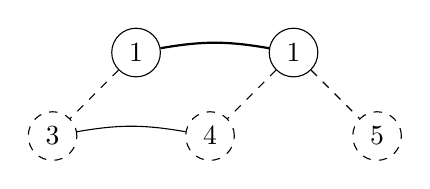
\begin{tikzpicture}[node distance={15mm}, table/.style = {draw,circle}, column/.style = {draw,dashed,circle}]

      \node[table] (users) at (0,0) {1}; 
      \node[table] (contacts) at (2,0) {1}; 
      
      \node[column] (users_id) [below left of=users] {3}; 
      
      \node[column] (contacts_user_id) [below left of=contacts] {4};
      \node[column] (contacts_name) [below right of=contacts] {5};
      
      \draw[dashed] (users) -- (users_id); 
      \draw[dashed] (contacts) -- (contacts_user_id); 
      \draw[dashed] (contacts) -- (contacts_name); 
      
      \draw[thick] (users) to [out=10, in=170] (contacts);
      
      \draw (users_id) to [out=10, in=170] (contacts_user_id); 
    \end{tikzpicture} 
    \caption{Normalized graph repr.}
    \label{figure:normalized-graph-representation}
  \end{minipage}
  \hfill
  \begin{minipage}[b]{0.45\linewidth}
    \centering
    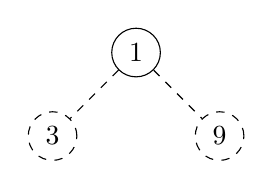
\begin{tikzpicture}[node distance={15mm}, table/.style = {draw,circle}, column/.style = {draw,dashed,circle}]
      \node[table] (users) at (0,0) {1}; 
      
      \node[column] (users_id) [below left of=users] {3}; 
      \node[column] (users_contacts) [below right of=users] {9};
      
      \draw[dashed] (users) -- (users_id); 
      \draw[dashed] (users) -- (users_contacts); 
    \end{tikzpicture} 
    \caption{Denormalized graph repr.}
    \label{figure:denormalized-graph-representation}
  \end{minipage}
  \hfill
  \vspace{1em}
  
  \begin{minipage}{\linewidth}
    \centering
    \vspace{0.5em}
    \small
    \textbf{Legend:} \cir{}~table~~\cir{dashed}~column~~\textbf{-}~foreign key~~--~reference~~- -~table-column
  \end{minipage}
\end{figure}

The $\delta$ of the order of the graphs~\ref{figure:normalized-graph-representation}
and~\ref{figure:denormalized-graph-representation}
further highlight the structural difference between the two schemas.

\paragraph{Distance Measurement}

To measure the distance between the graphs displayed in~\ref{figure:normalized-graph-representation}
and~\ref{figure:denormalized-graph-representation}, we employ the
Wasserstein Weisfeiler-Lehman (WWL) graph kernel method \citep{WWL}.

WWL kernels compute structural similarity by combining discrete Weisfeiler-Lehman
graph features with continuous optimal transport theory. The method first extracts
WL features from the labeled graph structure, then computes the Wasserstein distance
between the resulting feature distributions. For two graphs $G$ and
$G'$ with semantic node labels, the distance is computed as:

\begin{equation}
D^{f}_{W}(G, G') = W_1(f(G), f(G'))
\end{equation}

as introduced by \citeauthor{WWL} in \citeyear{WWL}.



For the database schemas above, the normalized schema (5 nodes, 5 edges) and
denormalized schema (3 nodes, 2 edges) show significant topological differences.
The WWL distance captures both the reduction in graph complexity (fewer nodes and edges)
and the loss of relational structure (elimination of foreign key relationships),
resulting in a substantial distance value reflecting their structural dissimilarity
despite representing equivalent logical data with $D^{f}_{W}(G_{norm}, G_{denorm}) \approx 0.78$.

% TODO: Clarify relationship between edge weights and WWL computation
% TODO: Add example showing how label priority affects similarity scores

\paragraph{Distance Index}

The distance index $d$ maintains precomputed distances between
all observed database schemas, enabling efficient retrieval of structurally similar
databases during sample selection. This index is constructed as a set of
schema-distance tuples $\{(sm_1, di_1), \ldots, (sm_i, di_i)\}$ where $sm_i$ is
a database schema name and $di_i$ denotes its WWL distance to the current schema.

% TODO: Fix inconsistent notation: use consistent variable names (G_s vs Natural-graphs)
% TODO: Improve transition between graph definition and distance measurement sections
